\documentclass[12pt, a4paper]{article}

\setlength{\parindent}{0pt}

% Packages essentiels
\usepackage[utf8]{inputenc}
\usepackage[T1]{fontenc}
\usepackage[french]{babel}
\usepackage{mathptmx} % Times New Roman
\usepackage{amsmath}
\usepackage{enumitem}
\usepackage{setspace}
\usepackage{fancyhdr}
\usepackage{titlesec}
\usepackage{pdfpages}
\usepackage{longtable}
\usepackage{booktabs}
\usepackage{array}
\usepackage{tabularx}
\usepackage{multirow}
\usepackage{parskip}

%highlight
\usepackage{soul}
\usepackage{xcolor}

%%%%%%%%%%%%%%%%%%%%%%%%%%%%%%%%%%%%%%%%%%%%%%%%%%%%%%%%%%%%%%%%%%%%%%%%%%%%%%%%%%%%%%%%%%
\usepackage{csquotes}
\usepackage{xurl}
\usepackage{hyperref}%[hidelinks]
\usepackage{apacite}

%%%%%%%%%%%%%%%%%%%%%%%%%%%%%%%%%%%%%%%%%%%%%%%%%%%%%%%%%%%%%%%%%%%%%%%%%%%%%%%%%%%%%%%%%%

% Marges : 2.5 cm gauche/droite, 3 cm haut/bas (avec pagination)
\usepackage[left=2.5cm, right=2.5cm, top=3cm, bottom=3cm]{geometry}

% Colonnes tabularx avec alignement à gauche pour éviter les underfull hbox
\newcolumntype{Y}{>{\raggedright\arraybackslash}X}

% Interligne 1.5
\onehalfspacing

% Correction headheight pour fancyhdr
\setlength{\headheight}{14.5pt}
\addtolength{\topmargin}{-2.5pt}

% Configuration de l'en-tête et pagination
\pagestyle{fancy}
\fancyhf{}
\fancyhead[R]{\thepage.}
\renewcommand{\headrulewidth}{0pt}
\renewcommand{\footrulewidth}{0pt}

% Subsubsection (alinéas) : italique
\titleformat{\subsubsection}
  {\normalfont\normalsize\itshape}{\thesubsubsection}{1em}{}

\begin{document}



% Page de garde
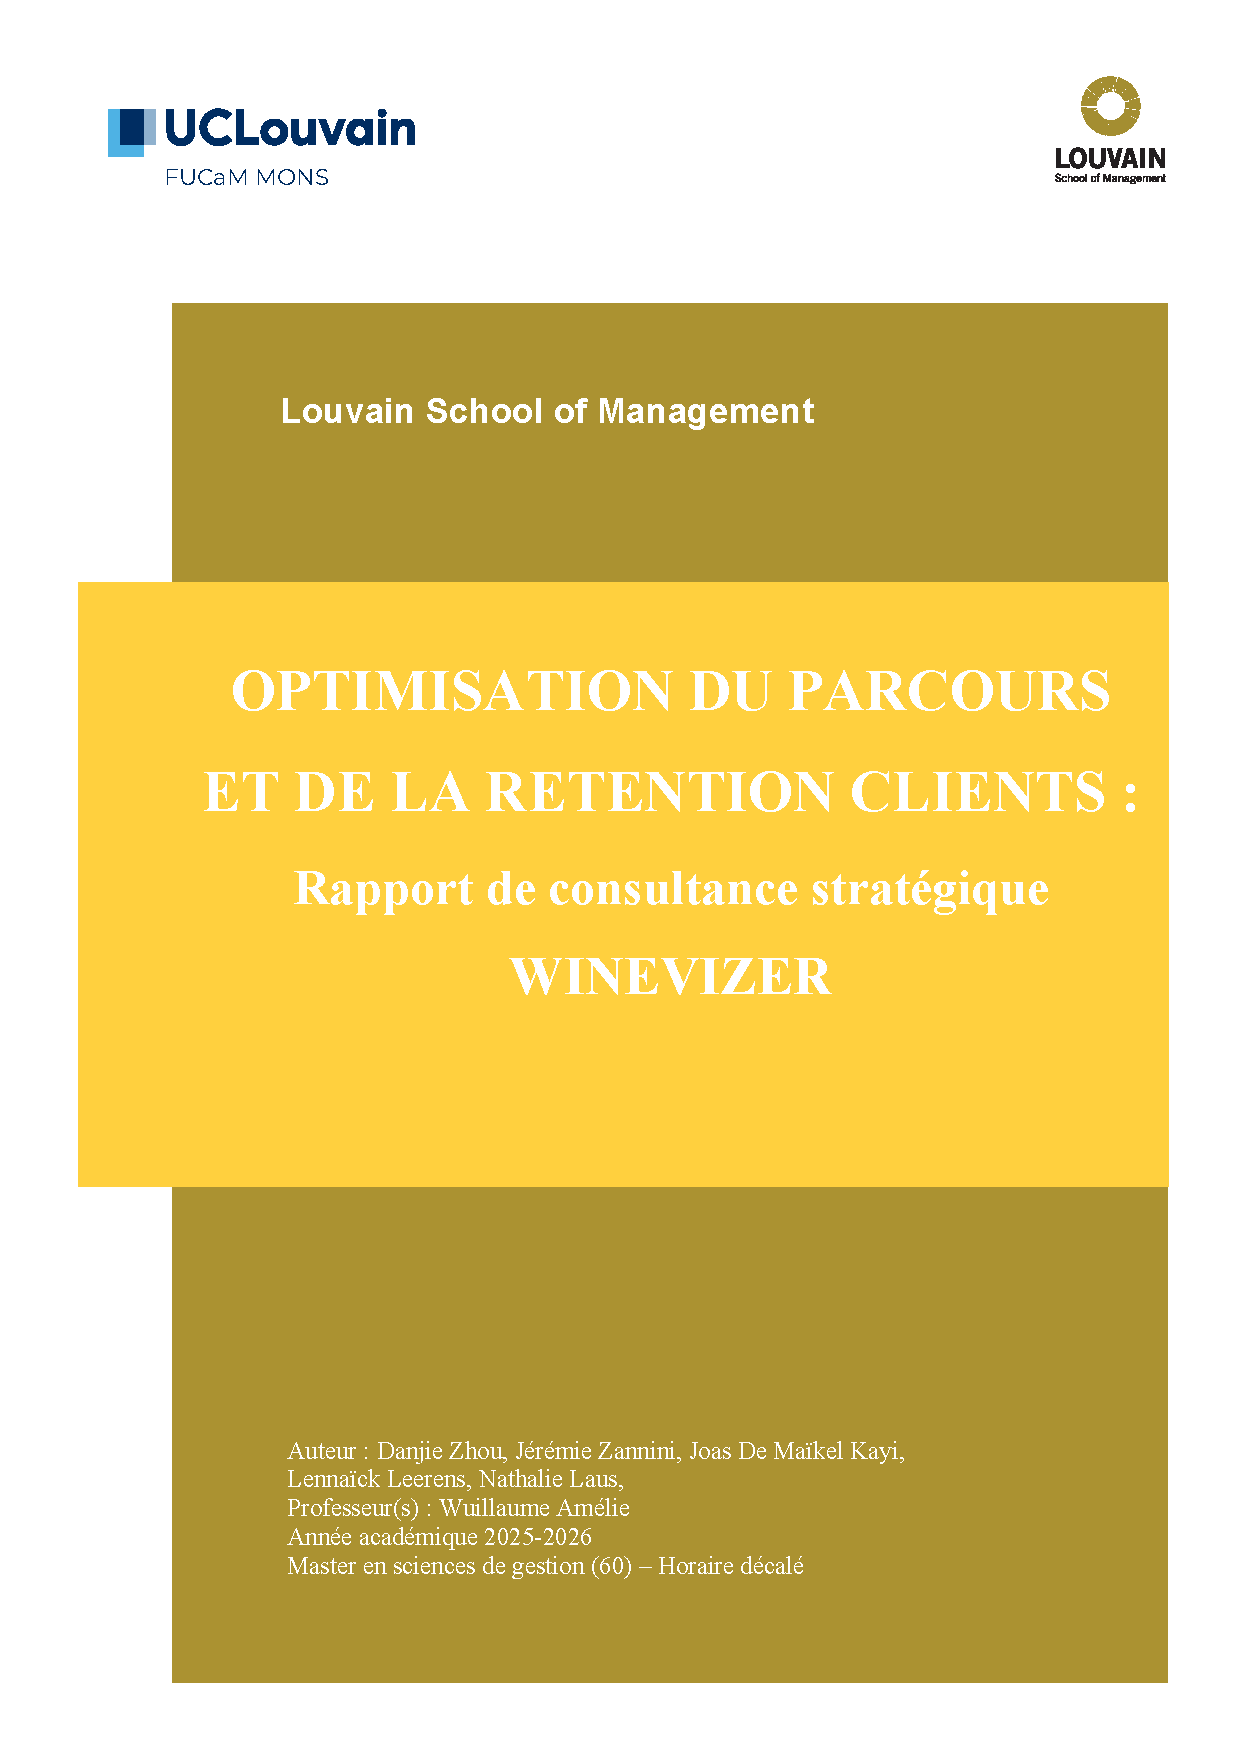
\includepdf[pages=-]{media/front.pdf}

\newpage
\tableofcontents

\newpage

\section{Introduction}

Le secteur de l'Horeca traverse aujourd'hui une phase de tensions structurelles. La crise du
Covid-19, suivie par la période post-Covid, a servi d'accélérateur en accentuant fortement ces
difficultés. À ce choc sanitaire s'est ajoutée une pression administrative et gouvernementale de
plus en plus lourde : le système de caisse enregistreuse obligatoire ou encore la gestion des
\og{}flexi-jobs\fg{} qui imposent un suivi rigoureux. Ces changements laissent de moins en moins de
temps aux restaurateurs pour gérer leur établissement \og{}en bon père de famille\fg{} et se concentrer
sur leur cœur de métier.

C'est dans ce contexte que s'inscrit Winevizer. Un environnement où les méthodes de
fonctionnement traditionnelles se heurtent à une nécessité de digitalisation subie. La
problématique est accentuée par la pénurie croissante de personnel qualifié, notamment de
sommeliers. Cette start-up wallonne lancée par Sébastien Demoustiez, propose une solution
SaaS (\textit{Software as a Service}) B2B (\textit{Business to Business}) innovante : une carte des vins digitale,
équipée d'un sommelier virtuel et présentée soit via un QR code, ou une tablette dans les
restaurants et les bars à vins.

L'ambition de Winevizer est de transformer des contraintes de gestion opérationnelles en un
véritable levier de rentabilité. Pour le restaurateur, Winevizer représente l'opportunité de
déléguer une partie de son travail à l'outil (la gestion du stock de la cave à vin, de la mise à
jour de la carte et \hl{une partie} du conseil d'un sommelier) pour vendre mieux et plus, tout en
offrant une expérience moderne et personnalisée aux clients de son établissement.

Malgré une proposition de valeur forte et une présence internationale, l'entreprise fait face à un
défi de taille : la rétention client lors de la phase d'\textbf{onboarding}, c'est-à-dire la phase où le
restaurateur doit configurer et enregistrer sa carte de vins dans l'outil. Près de 20\,\% des
utilisateurs abandonnent à ce stade. Pourquoi ?

Ce rapport analyse les causes de ce décrochage en explorant le parcours client, l'optimisation
du funnel de conversion et la lutte contre le \og{}churn\fg{} (taux d'attrition). En nous appuyant sur
l'entretien de Sébastien Demoustier, plus spécifiquement sur la situation décrite dans le cas
n°7, nous dresserons un diagnostic de l'entreprise et de son management, pour ensuite analyser
la problématique de la gestion de la relation client à l'aide des outils académiques adéquats.
Cette étude débouchera sur des recommandations stratégiques chiffrées et hiérarchisées, visant
à sécuriser et pérenniser le modèle économique de Winevizer.

\newpage
\section*{PARTIE 1 – DIAGNOSTIC : FOCUS SUR L'ENTREPRISE}
\addcontentsline{toc}{section}{Partie 1 – Diagnostic : Focus sur l'entreprise}

\section{Présentation générale de Winevizer}

Fondée durant les années Covid-19 (2021–2022) par Sébastien Demoustiez.

\vspace{0.5em}
\begin{tabularx}{\linewidth}{|>{\bfseries\raggedright\arraybackslash}p{4cm}|Y|}
  \hline
  Nom                              & Winevizer \\ \hline
  Site web                         & \url{www.winevizer.com} \\ \hline
  Fondateur                        & Sébastien Demoustiez – développeur freelance, entrepreneur wallon, \hl{$\sim$35 ans}. \\ \hline
  Siège                            & Mons, Wallonie, Belgique. \\ \hline
  Création                         & $\sim$2021. Lancée et développée durant la période Covid-19. \\ \hline
  Statut juridique et social       & Startup / PME – passage en société planifié en T1 2026 – Équipe réduite : 2 développeurs en activité complémentaire – recrutement d'un profil commercial prévu en 2026. \\ \hline
  Modèle économique                & SaaS B2B – abonnement 24,99\,€/mois ou 249,90\,€/an et par établissement Horeca. \\ \hline
  Concurrents identifiés           & Somm'it, Coena, Asterfox. \\ \hline
  Marchés principaux               & Benelux, France – UK, Canada, Danemark, Norvège, Australie, Malte. \\ \hline
  Objectifs commerciaux            & Objectif 2025 : Consolidation des 50 clients existants.\newline Objectif 2026 : 50 clients supplémentaires pour atteindre 100 clients – prospection de la grande distribution. \\ \hline
  C.A. annuel                      & $\sim$12\,000,00\,€ – Charges d'exploitation limitées à l'infrastructure IT. \\ \hline
  Taux d'attrition (churn)         & $\sim$10\,\% sur 3 ans (raisons principales : mauvaise situation financière ou fermeture de l'établissement client). \\ \hline
  Taux de conversion clients       & 20 à 25\,\% des utilisateurs qui ont encodé leur carte complète souscrivent l'abonnement. \\ \hline
  Canaux d'acquisition clients     & SEO (\textit{Search Engine Optimization}) : Top 3 sur Google\newline Bouche à oreille\newline Outbound : campagnes de pub, mailing, etc. : Coûts élevés et inefficaces. \\ \hline
\end{tabularx}

\section{La proposition de valeur}

Winevizer est une startup wallonne qui propose une solution SaaS B2B destinée au secteur
Horeca. La plateforme digitalise la carte des vins et propose les services d'un sommelier
virtuel, accessible via un QR code ou une tablette. Elle s'adresse exclusivement aux
professionnels (restaurants et bars à vins). Elle répond à une double exigence :

\begin{itemize}[leftmargin=1.5em]
  \item \textbf{Du côté du professionnel} (restaurateur ou bar à vin) : \hl{rotation importante de
        personnel, coût élevé et pénurie de personnel qualifié dans l'Horeca (sommeliers),
        recours à du personnel peu qualifié (étudiants, flexi-jobs) pour limiter les coûts et
        combler la rotation de personnel}, gestion complexe des cartes papier (liée à la gestion
        de stock et aux nouveautés, cartes multilingues), manque d'informations sur les
        préférences clients.

  \item \textbf{Du côté du consommateur final} : manque de connaissances en vins, peur du
        jugement du serveur, difficulté de faire un choix sur l'accord mets/vins.
\end{itemize}

Une fois connecté, le sommelier virtuel proposera d'accompagner le client de différentes
façons. La première possibilité est l'accord mets-vins ; la deuxième possibilité est une
sélection de vins par préférences gustatives (blanc, rouge, fruité, région, appellation, etc.).
La sélection sera toujours basée sur la liste des vins en stock. Les clients pourront alors
parcourir une série d'informations à propos du vin choisi comme par exemple la mise en
bouteille, de l'information sur le domaine, les notes attribuées par la communauté, etc.

\section{Management et profil entrepreneurial}

Winevizer est constituée de deux développeurs dont Sébastien Demoustiez, fondateur de
l'entreprise, qui assure le rôle à titre complémentaire de CEO, développeur, et bien qu'il
reconnaisse avoir bon nombre de lacunes dans ce domaine, il assure aussi la partie commerciale
et le support à la vente. Cette situation est à la fois une force et une faiblesse majeure :

\begin{itemize}[leftmargin=1.5em]
  \item \textbf{Force :} agilité liée à la startup, coûts faibles en masse salariale.
  \item \textbf{Faiblesse :} l'activité reste une activité complémentaire, ce qui ralentit le
        time-to-market. Les compétences commerciales sont limitées au \hl{démarrage} des nouveaux
        clients. L'engagement d'un profil commercial, à mi-temps, en T1~2026 (lors du passage
        en société) permettra une augmentation de la prospection et de la fidélisation clients
        et permettra une augmentation du CA de l'entreprise.
\end{itemize}

Actuellement, toutes les décisions produit s'appuient sur l'analyse des statistiques d'usage et
le fondateur adapte continuellement l'UX sur la base des retours clients.

\newpage
\section*{PARTIE 2 – DIAGNOSTIC : FOCUS SUR LA PROBLÉMATIQUE}
\addcontentsline{toc}{section}{Partie 2 – Diagnostic : Focus sur la problématique}

Pour répondre à la problématique de la rétention client lors de la phase d'onboarding durant
laquelle l'entreprise perd 20\,\% des utilisateurs, le choix s'est porté sur l'outil VPC –
\textit{Value Proposition Canvas}. Bien que le BMC – \textit{Business Model Canvas} offre une vision
holistique de l'entreprise, il s'avère être trop généraliste pour isoler les défaillances ou les
leviers opérationnels spécifiques. Le VPC permet d'effectuer une analyse ciblée sur
l'adéquation entre la proposition de valeur et les besoins réels du client. L'objectif n'est pas
de remettre en cause le modèle économique global, mais d'identifier le manque d'adéquation
(\textit{Mis-Fit}) qui survient dès la première interaction (technique) avec Winevizer.

\section{Analyse du profil client et de la proposition de valeur}

L'application du modèle représenté ci-dessous dans le Schéma~1 : \textit{Proposition de valeur /
profil de client} permet d'identifier les zones de friction suivantes.

\subsection{Le Profil du Client (\textit{Customer Profile})}

\begin{itemize}[leftmargin=1.5em]
  \item \textbf{Attentes du client (\textit{Customer Jobs}) :} Le restaurateur cherche à moderniser son
        conseil client et à digitaliser la gestion de stock de sa cave pour gagner en efficacité
        commerciale.

  \item \textbf{Frustrations (\textit{Pains}) :} Le principal frein identifié réside dans l'encodage manuel
        des références. Cette phase est perçue comme chronophage, techniquement complexe
        pour un public (Horeca) peu qualifié dans ce domaine et propice aux erreurs humaines.

  \item \textbf{Gains attendus (\textit{Gains}) :} Augmentation de l'addition ou du ticket moyen des
        clients du restaurant par le biais d'une meilleure vente croisée (mets-vins) et d'une
        synchronisation automatique de la carte avec les stocks réels de la cave à vins, sans
        coûts ni logistique supplémentaires liés à l'impression d'une carte papier.
\end{itemize}

\subsection{Proposition de Valeur (\textit{Value Proposition})}

\begin{itemize}[leftmargin=1.5em]
  \item \textbf{Produits \& services (\textit{Products \& services}) :} Grâce à une base de données qui
        répertorie la quasi-totalité des vins dans le monde, Winevizer facilite le conseil client
        en croisant les caractéristiques des vins présents sur la carte et des plats choisis par
        les clients.

  \item \textbf{Analgésiques (\textit{Pain relievers}) :} \hl{Pour réduire le taux d'attrition (churn) de 20\,\%
        des utilisateurs qui abandonnent la plateforme, Winevizer doit simplifier leur arrivée
        et automatiser l'étape d'onboarding (lecture automatique de PDF par l'IA). L'objectif
        est d'éliminer totalement l'effort de saisie pour convertir cette frustration critique
        en une expérience fluide.}

  \item \textbf{Générateurs de gains (\textit{Gains creators}) :} \hl{Winevizer crée de la valeur en
        renforçant la confiance du personnel de salle et en valorisant les stocks dormants
        grâce à la précision de l'algorithme de recommandation.}
\end{itemize}

\subsection{Synthèse : l'adéquation (le \textit{Fit}) comme levier de rétention}

Pour conclure ce premier diagnostic, l'analyse menée démontre que la proposition de valeur
de Winevizer est pertinente sur le fond grâce aux gains générés ; elle s'avère pourtant
déficiente sur la forme. Aujourd'hui, la pénibilité liée à l'onboarding est trop élevée \hl{trop affirmatatif selon moi,
on sait que 20\% stop au début mais est ce parce que c'est pénible ou c'est juste qu'ils ne voient pas la valeur ?
First impression last impression} lors de
la prise en main initiale. Pour assurer la rétention des utilisateurs, la priorité stratégique est
d'atteindre un \textit{Fit} technologique total. L'utilisateur ne doit plus percevoir l'application
Winevizer comme une charge de travail additionnelle, mais comme un assistant dont
l'installation est facilitée et l'usage est immédiat.

\section{La chaîne de valeur de Porter}

Pour compléter le diagnostic de la problématique vécue par Winevizer au niveau de
l'onboarding et de la rétention client, l'application de la chaîne de valeur de Porter présentée
en annexe est indispensable pour identifier les leviers et, plus spécifiquement, les points de
destruction de valeur dans le processus actuel. L'analyse démontre que le problème de
rétention se situe à l'intersection des activités primaires et de soutien :

\begin{itemize}[leftmargin=1.5em]
  \item \textbf{Activités Primaires (Logistique interne et Service) :} L'onboarding doit être
        considéré comme une phase de \og{}logistique interne\fg{} pour le client (l'intégration de
        l'outil dans son propre workflow). Si cette étape de support est trop contraignante, elle
        empêche le déploiement des activités suivantes : le marketing et la vente effective de
        vin auprès du client final.

  \item \textbf{Activités de soutien (R\&D et infrastructure) :} \hl{Winevizer dispose d'un avantage
        concurrentiel important grâce à sa base de données sémantique. Toutefois, la
        \og{}technologie d'accès\fg{} (interface d'encodage) constitue actuellement une barrière à
        l'entrée. Comme illustré par le cas Benetton, étudié en cours, la performance d'une PME
        repose sur l'efficience de ses systèmes d'information (SI). Ici, le SI est expert sur
        le fond mais totalement inefficient dans sa modalité d'accès.}
\end{itemize}

\subsection{Impact sur la marge et la création/destruction de valeur}

Le modèle de la chaîne de valeur permet de comprendre que la marge est le résultat de
l'ensemble des activités. Dans notre cas, l'abandon de 20\,\% des clients au moment de
l'onboarding constitue donc une destruction de valeur critique :

\begin{itemize}[leftmargin=1.5em]
  \item \textbf{Coût d'acquisition perdu :} les ressources mobilisées pour attirer le client
        deviennent une perte sèche puisque ce dernier abandonne l'outil avant même
        l'utilisation réelle et surtout avant même que l'entreprise n'ait réalisé de bénéfice.

  \item \textbf{Goulot d'étranglement opérationnel :} l'encodage manuel des cartes agit comme un
        goulot d'étranglement et paralyse la proposition de valeur. \hl{pas plutot qu'on arrive trop tard à l'encodage ?}
\end{itemize}

\section{Conclusion du diagnostic : Matrice SWOT}

La matrice SWOT permet de croiser les variables internes à Winevizer (issues du VRIO et de
la chaîne de valeur, présentés en annexe) avec les facteurs d'influence de son environnement
(issus du PESTEL et des 5 forces~+~1 de Porter présentés en annexe). Cette synthèse sert de
fondement à la stratégie de rétention et permet d'isoler le levier technologique capable de
neutraliser la perte d'utilisateurs.

\vspace{1em}
\begin{tabularx}{\linewidth}{|Y|Y|}
  \hline
  \multicolumn{1}{|c|}{\textbf{FORCES (\textit{Strengths})}} &
  \multicolumn{1}{c|}{\textbf{FAIBLESSES (\textit{Weaknesses})}} \\
  \hline
  \begin{itemize}[leftmargin=1em, topsep=2pt, itemsep=1pt]
    \item Sommelier virtuel contextuel unique sur le marché européen
    \item Algorithme de recommandation (accords mets-vins + préférences aromatiques)
    \item Base de données sémantique (95\,\% des vins mondiaux)
    \item Référencement SEO exceptionnel (Top 3 sur mots clés stratégiques)
    \item Modèle SaaS léger, faibles coûts fixes
    \item Solution multilingue (7 langues) — atout international
    \item Taux de churn faible (10\,\%)
    \item IA intégrée (pour les cartes PDF, génération de contenu SEO)
    \item Données comportementales clients accumulées sur 3 ans
    \item Prix d'entrée compétitif (24,99\,€/mois) – faible barrière à l'adoption
  \end{itemize} &
  \begin{itemize}[leftmargin=1em, topsep=2pt, itemsep=1pt]
    \item Équipe limitée à 2 personnes, pas de force commerciale
    \item Activité complémentaire – manque de temps et de focus stratégique
    \item C.A. annuel insuffisant pour rendre le modèle viable à LT ($\sim$12\,000\,€)
    \item Absence de protection IP (algorithme non breveté, base de données non protégée)
    \item Prospection commerciale quasi-inexistante
    \item Taux de conversion du funnel faible (pertes à chaque étape)
    \item Outbound marketing peu efficace (mailing, Google Ads)
    \item Pas encore en société – frein à la crédibilité et aux financements
    \item Peu d'intégrations POS par rapport à Somm'it
  \end{itemize} \\
  \hline
  \multicolumn{1}{|c|}{\textbf{OPPORTUNITÉS (\textit{Opportunities})}} &
  \multicolumn{1}{c|}{\textbf{MENACES (\textit{Threats})}} \\
  \hline
  \begin{itemize}[leftmargin=1em, topsep=2pt, itemsep=1pt]
    \item Marché US porteur (technophile, prix peu sensible, sans prospection active)
    \item Extension à la grande distribution (rayons vins en GMS), ticket moyen élevé potentiel
    \item Passage en société – accès aux primes publiques et crédibilité
    \item Tendance no/low alcohol – extension vers les softs et mocktails
    \item E-label règlementaire UE – démocratisation du QR code œnologique
    \item Partenariats prescripteurs (écoles de cuisine, sommeliers, cavistes, fournisseurs Horeca)
    \item Modèle freemium, plans tarifaires différenciés – hausse ARPU
    \item Digitalisation accélérée du secteur Horeca post-Covid
    \item Recrutement d'un profil commercial – accélération de la croissance
  \end{itemize} &
  \begin{itemize}[leftmargin=1em, topsep=2pt, itemsep=1pt]
    \item IA générative – imitation rapide de la solution (menace principale identifiée)
    \item Concurrents US potentiellement mieux financés et technologiques
    \item Résistance culturelle française à la digitalisation du vin
    \item Dépendance au SEO comme unique canal d'acquisition
    \item Volatilité EUR/USD – risque de perte sur facturation en dollars
    \item Protectionnisme américain (Trump) – incertitude sur services numériques
    \item Concentration des fondateurs – risque humain critique
    \item Adoption insuffisante en UK (résistance au QR code)
    \item Montée en gamme de Somm'it vers les petits restaurants
    \item Saturation de l'espace SEO par des concurrents mieux dotés en contenu IA
  \end{itemize} \\
  \hline
\end{tabularx}

\newpage
\appendix
\section{Annexe 1 : Chaîne de valeur}

La chaîne de valeur de Winevizer identifie les activités créatrices de valeur et celles à
externaliser ou à développer.

\vspace{1em}
\begin{tabularx}{\linewidth}{|>{\bfseries\raggedright\arraybackslash}p{4cm}|Y|>{\centering\arraybackslash}p{3cm}|}
  \hline
  \textbf{Activité} & \textbf{Description} & \textbf{Valeur créée} \\
  \hline
  \multicolumn{3}{|l|}{\textbf{ACTIVITÉS PRIMAIRES}} \\
  \hline
  Logistique interne &
  Onboarding client : importation des cartes, encodage de la carte via IA/OCR, import Excel. &
  $\downarrow$ (point de rupture) \\
  \hline
  Opérations &
  Fonctionnement de l'app (iOS/Android), génération des recommandations en temps réel, intégration POS. &
  $\uparrow\uparrow\uparrow\uparrow\uparrow$ \\
  \hline
  Logistique externe &
  Mise à disposition de la carte digitale via QR code/tablette pour les clients finaux. &
  $\uparrow\uparrow\uparrow\uparrow$ \\
  \hline
  Vente \& Marketing &
  SEO organique et bouche à oreille efficaces, manque de prospection active, campagnes publicitaires peu efficaces (dépendance à l'inbound). &
  $\uparrow\uparrow\uparrow$ (SEO)\newline $\uparrow$ (Ads) \\
  \hline
  SAV &
  Réponses aux questions, accompagnement des restaurateurs, facteur de rétention. &
  $\uparrow\uparrow\uparrow\uparrow$ \\
  \hline
  \multicolumn{3}{|l|}{\textbf{ACTIVITÉS DE SOUTIEN}} \\
  \hline
  Infrastructure \& IT &
  Hébergement cloud green, disponibilité et performance. Coûts maîtrisés. &
  $\uparrow\uparrow\uparrow\uparrow$ \\
  \hline
  Gestion RH &
  Équipe technique (2 développeurs), recrutement imminent d'un commercial. Lacune critique actuelle. &
  $\uparrow\uparrow$ (Vulnérabilité) \\
  \hline
  Développement technologique (R\&D) &
  Codage de l'algorithme, maintenance et enrichissement de la base de données (95\,\% du marché), intégration continue de l'IA/OCR pour PDF, nouvelles fonctionnalités, roadmap produit. Cœur de l'activité. &
  $\uparrow\uparrow\uparrow\uparrow\uparrow$ \\
  \hline
  Achats / Approvisionnements &
  Gestion des licences logicielles et des flux de données externes. &
  $\uparrow\uparrow\uparrow$ \\
  \hline
\end{tabularx}







\nocite{*}
\bibliographystyle{apacite}
\bibliography{references}


\includepdf[pages=-]{media/back.pdf}

\end{document}
